\documentclass[12pt,a4paper]{article}

\usepackage[a4paper,text={16.5cm,25.2cm},centering]{geometry}
\usepackage{lmodern}
\usepackage{amssymb,amsmath}
\usepackage{bm}
\usepackage{graphicx}
\usepackage{microtype}
\usepackage{hyperref}
\setlength{\parindent}{0pt}
\setlength{\parskip}{1.2ex}

\hypersetup
       {   pdfauthor = { Marco Fasondini },
           pdftitle={ foo },
           colorlinks=TRUE,
           linkcolor=black,
           citecolor=blue,
           urlcolor=blue
       }




\usepackage{upquote}
\usepackage{listings}
\usepackage{xcolor}
\lstset{
    basicstyle=\ttfamily\footnotesize,
    upquote=true,
    breaklines=true,
    breakindent=0pt,
    keepspaces=true,
    showspaces=false,
    columns=fullflexible,
    showtabs=false,
    showstringspaces=false,
    escapeinside={(*@}{@*)},
    extendedchars=true,
}
\newcommand{\HLJLt}[1]{#1}
\newcommand{\HLJLw}[1]{#1}
\newcommand{\HLJLe}[1]{#1}
\newcommand{\HLJLeB}[1]{#1}
\newcommand{\HLJLo}[1]{#1}
\newcommand{\HLJLk}[1]{\textcolor[RGB]{148,91,176}{\textbf{#1}}}
\newcommand{\HLJLkc}[1]{\textcolor[RGB]{59,151,46}{\textit{#1}}}
\newcommand{\HLJLkd}[1]{\textcolor[RGB]{214,102,97}{\textit{#1}}}
\newcommand{\HLJLkn}[1]{\textcolor[RGB]{148,91,176}{\textbf{#1}}}
\newcommand{\HLJLkp}[1]{\textcolor[RGB]{148,91,176}{\textbf{#1}}}
\newcommand{\HLJLkr}[1]{\textcolor[RGB]{148,91,176}{\textbf{#1}}}
\newcommand{\HLJLkt}[1]{\textcolor[RGB]{148,91,176}{\textbf{#1}}}
\newcommand{\HLJLn}[1]{#1}
\newcommand{\HLJLna}[1]{#1}
\newcommand{\HLJLnb}[1]{#1}
\newcommand{\HLJLnbp}[1]{#1}
\newcommand{\HLJLnc}[1]{#1}
\newcommand{\HLJLncB}[1]{#1}
\newcommand{\HLJLnd}[1]{\textcolor[RGB]{214,102,97}{#1}}
\newcommand{\HLJLne}[1]{#1}
\newcommand{\HLJLneB}[1]{#1}
\newcommand{\HLJLnf}[1]{\textcolor[RGB]{66,102,213}{#1}}
\newcommand{\HLJLnfm}[1]{\textcolor[RGB]{66,102,213}{#1}}
\newcommand{\HLJLnp}[1]{#1}
\newcommand{\HLJLnl}[1]{#1}
\newcommand{\HLJLnn}[1]{#1}
\newcommand{\HLJLno}[1]{#1}
\newcommand{\HLJLnt}[1]{#1}
\newcommand{\HLJLnv}[1]{#1}
\newcommand{\HLJLnvc}[1]{#1}
\newcommand{\HLJLnvg}[1]{#1}
\newcommand{\HLJLnvi}[1]{#1}
\newcommand{\HLJLnvm}[1]{#1}
\newcommand{\HLJLl}[1]{#1}
\newcommand{\HLJLld}[1]{\textcolor[RGB]{148,91,176}{\textit{#1}}}
\newcommand{\HLJLs}[1]{\textcolor[RGB]{201,61,57}{#1}}
\newcommand{\HLJLsa}[1]{\textcolor[RGB]{201,61,57}{#1}}
\newcommand{\HLJLsb}[1]{\textcolor[RGB]{201,61,57}{#1}}
\newcommand{\HLJLsc}[1]{\textcolor[RGB]{201,61,57}{#1}}
\newcommand{\HLJLsd}[1]{\textcolor[RGB]{201,61,57}{#1}}
\newcommand{\HLJLsdB}[1]{\textcolor[RGB]{201,61,57}{#1}}
\newcommand{\HLJLsdC}[1]{\textcolor[RGB]{201,61,57}{#1}}
\newcommand{\HLJLse}[1]{\textcolor[RGB]{59,151,46}{#1}}
\newcommand{\HLJLsh}[1]{\textcolor[RGB]{201,61,57}{#1}}
\newcommand{\HLJLsi}[1]{#1}
\newcommand{\HLJLso}[1]{\textcolor[RGB]{201,61,57}{#1}}
\newcommand{\HLJLsr}[1]{\textcolor[RGB]{201,61,57}{#1}}
\newcommand{\HLJLss}[1]{\textcolor[RGB]{201,61,57}{#1}}
\newcommand{\HLJLssB}[1]{\textcolor[RGB]{201,61,57}{#1}}
\newcommand{\HLJLnB}[1]{\textcolor[RGB]{59,151,46}{#1}}
\newcommand{\HLJLnbB}[1]{\textcolor[RGB]{59,151,46}{#1}}
\newcommand{\HLJLnfB}[1]{\textcolor[RGB]{59,151,46}{#1}}
\newcommand{\HLJLnh}[1]{\textcolor[RGB]{59,151,46}{#1}}
\newcommand{\HLJLni}[1]{\textcolor[RGB]{59,151,46}{#1}}
\newcommand{\HLJLnil}[1]{\textcolor[RGB]{59,151,46}{#1}}
\newcommand{\HLJLnoB}[1]{\textcolor[RGB]{59,151,46}{#1}}
\newcommand{\HLJLoB}[1]{\textcolor[RGB]{102,102,102}{\textbf{#1}}}
\newcommand{\HLJLow}[1]{\textcolor[RGB]{102,102,102}{\textbf{#1}}}
\newcommand{\HLJLp}[1]{#1}
\newcommand{\HLJLc}[1]{\textcolor[RGB]{153,153,119}{\textit{#1}}}
\newcommand{\HLJLch}[1]{\textcolor[RGB]{153,153,119}{\textit{#1}}}
\newcommand{\HLJLcm}[1]{\textcolor[RGB]{153,153,119}{\textit{#1}}}
\newcommand{\HLJLcp}[1]{\textcolor[RGB]{153,153,119}{\textit{#1}}}
\newcommand{\HLJLcpB}[1]{\textcolor[RGB]{153,153,119}{\textit{#1}}}
\newcommand{\HLJLcs}[1]{\textcolor[RGB]{153,153,119}{\textit{#1}}}
\newcommand{\HLJLcsB}[1]{\textcolor[RGB]{153,153,119}{\textit{#1}}}
\newcommand{\HLJLg}[1]{#1}
\newcommand{\HLJLgd}[1]{#1}
\newcommand{\HLJLge}[1]{#1}
\newcommand{\HLJLgeB}[1]{#1}
\newcommand{\HLJLgh}[1]{#1}
\newcommand{\HLJLgi}[1]{#1}
\newcommand{\HLJLgo}[1]{#1}
\newcommand{\HLJLgp}[1]{#1}
\newcommand{\HLJLgs}[1]{#1}
\newcommand{\HLJLgsB}[1]{#1}
\newcommand{\HLJLgt}[1]{#1}



\def\qqand{\qquad\hbox{and}\qquad}
\def\qqfor{\qquad\hbox{for}\qquad}
\def\qqas{\qquad\hbox{as}\qquad}
\def\half{ {1 \over 2} }
\def\D{ {\rm d} }
\def\I{ {\rm i} }
\def\E{ {\rm e} }
\def\C{ {\mathbb C} }
\def\R{ {\mathbb R} }
\def\bbR{ {\mathbb R} }
\def\H{ {\mathbb H} }
\def\Z{ {\mathbb Z} }
\def\CC{ {\cal C} }
\def\FF{ {\cal F} }
\def\HH{ {\cal H} }
\def\LL{ {\cal L} }
\def\vc#1{ {\mathbf #1} }
\def\bbC{ {\mathbb C} }



\def\fR{ f_{\rm R} }
\def\fL{ f_{\rm L} }

\def\qqqquad{\qquad\qquad}
\def\qqwhere{\qquad\hbox{where}\qquad}
\def\Res_#1{\underset{#1}{\rm Res}\,}
\def\sech{ {\rm sech}\, }
\def\acos{ {\rm acos}\, }
\def\asin{ {\rm asin}\, }
\def\atan{ {\rm atan}\, }
\def\Ei{ {\rm Ei}\, }
\def\upepsilon{\varepsilon}


\def\Xint#1{ \mathchoice
   {\XXint\displaystyle\textstyle{#1} }%
   {\XXint\textstyle\scriptstyle{#1} }%
   {\XXint\scriptstyle\scriptscriptstyle{#1} }%
   {\XXint\scriptscriptstyle\scriptscriptstyle{#1} }%
   \!\int}
\def\XXint#1#2#3{ {\setbox0=\hbox{$#1{#2#3}{\int}$}
     \vcenter{\hbox{$#2#3$}}\kern-.5\wd0} }
\def\ddashint{\Xint=}
\def\dashint{\Xint-}
% \def\dashint
\def\infdashint{\dashint_{-\infty}^\infty}




\def\addtab#1={#1\;&=}
\def\ccr{\\\addtab}
\def\ip<#1>{\left\langle{#1}\right\rangle}
\def\dx{\D x}
\def\dt{\D t}
\def\dz{\D z}
\def\ds{\D s}

\def\rR{ {\rm R} }
\def\rL{ {\rm L} }

\def\norm#1{\left\| #1 \right\|}

\def\pr(#1){\left({#1}\right)}
\def\br[#1]{\left[{#1}\right]}

\def\abs#1{\left|{#1}\right|}
\def\fpr(#1){\!\pr({#1})}

\def\sopmatrix#1{ \begin{pmatrix}#1\end{pmatrix} }

\def\endash{–}
\def\emdash{—}
\def\mdblksquare{\blacksquare}
\def\lgblksquare{\blacksquare}
\def\scre{\E}
\def\mapengine#1,#2.{\mapfunction{#1}\ifx\void#2\else\mapengine #2.\fi }

\def\map[#1]{\mapengine #1,\void.}

\def\mapenginesep_#1#2,#3.{\mapfunction{#2}\ifx\void#3\else#1\mapengine #3.\fi }

\def\mapsep_#1[#2]{\mapenginesep_{#1}#2,\void.}


\def\vcbr[#1]{\pr(#1)}


\def\bvect[#1,#2]{
{
\def\dots{\cdots}
\def\mapfunction##1{\ | \  ##1}
	\sopmatrix{
		 \,#1\map[#2]\,
	}
}
}



\def\vect[#1]{
{\def\dots{\ldots}
	\vcbr[{#1}]
} }

\def\vectt[#1]{
{\def\dots{\ldots}
	\vect[{#1}]^{\top}
} }

\def\Vectt[#1]{
{
\def\mapfunction##1{##1 \cr}
\def\dots{\vdots}
	\begin{pmatrix}
		\map[#1]
	\end{pmatrix}
} }

\def\addtab#1={#1\;&=}
\def\ccr{\\\addtab}

\def\questionequals{= \!\!\!\!\!\!{\scriptstyle ? \atop }\,\,\,}

\def\Ei{\rm Ei\,}

\begin{document}

\section{Chapter 5: Exercises Solutions}
Consider the following finite difference method for the diffusion equation

\[
-\frac{1}{2}\mu u^{i+1}_{j-1} + (1 + \mu)u^{i+1}_j -\frac{1}{2}\mu u^{i+1}_{j+1} = 
\frac{1}{2}\mu u^{i}_{j-1} + (1 - \mu)u^{i}_j +\frac{1}{2}\mu u^{i}_{j+1} 
\]
where $\mu = \tau/h^2$.

\begin{itemize}
\item[1. ] Show that the method has a second-order local truncation error. That is, let $\tilde{u}^i_j = u(x_j,t_i)$, where $x_j = jh$, $t_i = i\tau$, show that the method can be expressed as

\end{itemize}
\[
\frac{u^{i+1}_j - u^i_j}{\tau} = \frac{1}{2}\left( \frac{u^{i+1}_{j+1} - 2u^{i+1}_{j} + u^{i+1}_{j-1}}{h^2} + \frac{u^{i}_{j+1} - 2u^{i}_{j} + u^{i}_{j-1}}{h^2}   \right)
\]
and then show that for $\tau, h \to 0$ (assuming all the relevant partial derivatives are bounded),


\begin{eqnarray*}
&& \frac{\tilde{u}^{i+1}_j - \tilde{u}^i_j}{\tau} - \frac{1}{2}\left( \frac{\tilde{u}^{i+1}_{j+1} - 2\tilde{u}^{i+1}_{j} + \tilde{u}^{i+1}_{j-1}}{h^2} + \frac{\tilde{u}^{i}_{j+1} - 2\tilde{u}^{i}_{j} + \tilde{u}^{i}_{j-1}}{h^2}   \right) = \mathcal{O}(\tau^2) + \mathcal{O}(h^2).
\end{eqnarray*}
Hint: use Taylor's theorem to expand the exact solution about $(x,t) = (x_j,t_{i+1/2})$, where $t_{i+1/2} = (i + 1/2)\tau = t_i + \tau/2$.

\textbf{Solution} The method can be expressed as

\[
\frac{u^{i+1}_j - u^i_j}{\tau} = \frac{1}{2}\left( \frac{u^{i+1}_{j+1} - 2u^{i+1}_{j} + u^{i+1}_{j-1}}{h^2} + \frac{u^{i}_{j+1} - 2u^{i}_{j} + u^{i}_{j-1}}{h^2}   \right).
\]
Using Taylor's theorem to expand the solution about $(x_j, t_{i+1/2})$, we have that as $\tau \to 0$,


\begin{eqnarray*}
\tilde{u}^{i+1}_j  &=& u(x_{j},t_{i+1}) \\
                 &=& u(x_j,t_{i+1/2}+\tau/2) \\
                 &=& u(x_j,t_{i+1/2}) + \frac{\tau}{2}u_t(x_j,t_{i+1/2}) + \frac{\tau^2}{8}u_{tt}(x_j,t_{i+1/2}) + \mathcal{O}(\tau^3)
\end{eqnarray*}
and similarly


\begin{eqnarray*}
\tilde{u}^{i}_j  &=& u(x_{j},t_{i})\\
                 &=& u(x_j,t_{i+1/2}-\tau/2) \\
                 &=& u(x_j,t_{i+1/2}) - \frac{\tau}{2}u_t(x_j,t_{i+1/2}) + \frac{\tau^2}{8}u_{tt}(x_j,t_{i+1/2}) + \mathcal{O}(\tau^3)
\end{eqnarray*}
Therefore,

\[
\frac{\tilde{u}^{i+1}_j - \tilde{u}^i_j}{\tau} = u_t(x_j,t_{i+1/2}) + \mathcal{O}(\tau^2)
\]
We have shown in the lecture notes (using Taylor's theorem) that

\[
\frac{\tilde{u}^{i}_{j+1} - 2\tilde{u}^{i}_{j} + \tilde{u}^{i}_{j-1}}{h^2} = u_{xx}(x_j,t_i) + \mathcal{O}(h^2),
\]
therefore, using Taylor's theorem again, but in the time variable,


\begin{eqnarray*}
\frac{\tilde{u}^{i}_{j+1} - 2\tilde{u}^{i}_{j} + \tilde{u}^{i}_{j-1}}{h^2} &=& u_{xx}(x_j,t_i) + \mathcal{O}(h^2)  \\
&=&  u_{xx}(x_j,t_{i+1/2}-\tau/2) + \mathcal{O}(h^2) \\
&=&  u_{xx}(x_j,t_{i+1/2}) - \frac{\tau}{2}u_{txx}(x_j,t_{i+1/2}) +  \mathcal{O}(\tau^2) + \mathcal{O}(h^2).
\end{eqnarray*}
Similarly,


\begin{eqnarray*}
\frac{\tilde{u}^{i+1}_{j+1} - 2\tilde{u}^{i+1}_{j} + \tilde{u}^{i+1}_{j-1}}{h^2} &=& u_{xx}(x_j,t_{i+1}) + \mathcal{O}(h^2)  \\
&=&  u_{xx}(x_j,t_{i+1/2}+\tau/2) + \mathcal{O}(h^2) \\
&=&  u_{xx}(x_j,t_{i+1/2}) + \frac{\tau}{2}u_{txx}(x_j,t_{i+1/2}) +  \mathcal{O}(\tau^2) + \mathcal{O}(h^2)
\end{eqnarray*}
and hence


\begin{eqnarray*}
&& \frac{\tilde{u}^{i+1}_j - \tilde{u}^i_j}{\tau} - \frac{1}{2}\left( \frac{\tilde{u}^{i+1}_{j+1} - 2\tilde{u}^{i+1}_{j} + \tilde{u}^{i+1}_{j-1}}{h^2} + \frac{\tilde{u}^{i}_{j+1} - 2\tilde{u}^{i}_{j} + \tilde{u}^{i}_{j-1}}{h^2}   \right) \\
&& =  u_t(x_j,t_{i+1/2}) - u_{xx}(x_j,t_{i+1/2})  +  \mathcal{O}(\tau^2) + \mathcal{O}(h^2) \\
&& = \mathcal{O}(\tau^2) + \mathcal{O}(h^2)
\end{eqnarray*}
\begin{itemize}
\item[2. ] Use the Von Neumann method to show that the method is unconditionally stable.

\end{itemize}
\textbf{Solution} Setting $u^{i}_j = \lambda^i {\rm e}^{{\rm i}kx_j}$ in

\[
-\frac{1}{2}\mu u^{i+1}_{j-1} + (1 + \mu)u^{i+1}_j -\frac{1}{2}\mu u^{i+1}_{j+1} = 
\frac{1}{2}\mu u^{i}_{j-1} + (1 - \mu)u^{i}_j +\frac{1}{2}\mu u^{i}_{j+1} 
\]
we find that

\[
\lambda\left[1 - \frac{\mu}{2}\left({\rm e}^{-{\rm i}kh} - 2 +  {\rm e}^{{\rm i}kh} \right)    \right] = 1 + \frac{\mu}{2}\left({\rm e}^{-{\rm i}kh} - 2 +  {\rm e}^{{\rm i}kh} \right)  
\]
and since $\left({\rm e}^{-{\rm i}kh} - 2 +  {\rm e}^{{\rm i}kh} \right) = \left({\rm e}^{-{\rm i}kh/2} -  {\rm e}^{{\rm i}kh/2} \right)^2 = -4\sin^2(kh/2)$, it follows that

\[
\lambda = \frac{1 - 2\mu\sin^2(kh/2)}{1 + 2\mu\sin^2(kh/2)}
\]
Since $\vert 1 - 2\mu\sin^2(kh/2) \vert \leq \vert 1 + 2\mu\sin^2(kh/2)\vert$ for $\mu > 0$, $k \in \mathbb{Z}$ and $h > 0$, it follows that $\vert \lambda \vert \leq 1$ for these same parameter values and therefore the method is unconditionally stable.

\begin{itemize}
\item[3. ] Suppose the finite difference method is used to approximate the solution to the diffusion equation $u_t = u_{xx}$ for $(x, t) \in (0,1) \times (0,T)$ subject to $u(0,t) = \varphi_0(t)$, $u(1,t) = \varphi_1(t)$ for $t \in [0, T]$ and $u(x,0) = f(x)$ for $x \in [0, 1]$.  Let $u(x_j,t_i) \approx u^i_j$, where $x_j = jh$, $h = 1/(n_x + 1)$, $j = 0, \ldots, n_x+1$, $t_i = i\tau$, $\tau = \mu h^2$ and set

\end{itemize}
\[
\mathbf{u}^i = \begin{bmatrix}
u^{i}_{1} \\
\vdots \\
u^{i}_{n_x}
\end{bmatrix} \in \mathbb{R}^{n_x}.
\]
The finite difference method can be expressed as

\[
L\mathbf{u}^{i+1} = R\mathbf{u}^{i} + \mathbf{k}^{i},
\]
where $L, R \in \mathbb{R}^{n_x \times n_x}$ and $\mathbf{k}^{i} \in \mathbb{R}^{n_x}$.  Give the matrices $L$ and $R$ and the vector $\mathbf{k}^{i}$.

\textbf{Solution}


\begin{eqnarray*}
&&
\underbrace{\begin{bmatrix}
1 + \mu & -\mu/2 & & & \\
-\mu/2  & 1+\mu & -\mu/2  & & \\
      & \ddots & \ddots & \ddots & \\
      &        & -\mu/2    & 1+ \mu & -\mu/2 \\
      &        &        &-\mu/2      & 1+\mu
\end{bmatrix}}_{L}
\underbrace{\begin{bmatrix}
u^{i+1}_{1} \\
\vdots \\
\vdots \\
\vdots \\
u^{i+1}_{n_x}
\end{bmatrix}}_{\mathbf{u}^{i+1}} = \\
&& 
\underbrace{\begin{bmatrix}
1 - \mu & \mu/2 & & & \\
\mu/2  & 1-\mu & \mu/2  & & \\
      & \ddots & \ddots & \ddots & \\
      &        & \mu/2    & 1- \mu & \mu/2 \\
      &        &        &\mu/2      & 1-\mu
\end{bmatrix}}_{R}
\underbrace{\begin{bmatrix}
u^{i}_{1} \\
\vdots \\
\vdots \\
\vdots \\
u^{i}_{n_x}
\end{bmatrix}}_{\mathbf{u}^i}
+
\underbrace{\begin{bmatrix}
\mu(\varphi_0(t_i) + \varphi_0(t_{i+1}))/2 \\
0 \\
\vdots \\
0 \\
\mu(\varphi_1(t_i) + \varphi_1(t_{i+1}))/2
\end{bmatrix}}_{\mathbf{k}^i}
\end{eqnarray*}
\begin{itemize}
\item[4. ] What are the eigenvalues of the matrix $A := L^{-1}R$? Find a bound on the spectral radius of $A$.   Hint: consider the eigendecomposition (spectral factorisation) of $L$ and $R$.

\end{itemize}
\textbf{Solution} The matrices $L$ and $R$ are TST (Tridiagonal, symmetric, Toeplitz); from the notes we know that an $n_x \times n_x$ TST matrix with $\alpha$ on the main diagonal and $\beta$ on the super and subdiagonals have eigenvalues 

\[
\lambda_j = \alpha + 2\beta\cos\left( \frac{\pi j}{n_x+1}  \right), \qquad j = 1, \ldots, n_x.
\]
Therefore, for $j = 1, \ldots, n_x$, the eigenvalues of $L$ are

\[
\lambda_j^{L} = 1 + \mu - \mu \cos\left(\pi x_j  \right) =  1 + \mu - \mu\left(1 - 2\sin^2\left(\pi x_j /2 \right)\right) = 1 + 2\mu\sin^2(\pi x_j/2)
\]
and those of $R$ are

\[
\lambda_j^{R} = 1 - \mu + \mu \cos\left(\pi x_j  \right) =  1 - \mu + \mu\left(1 - 2\sin^2\left(\pi x_j /2 \right)\right) = 1 - 2\mu\sin^2(\pi x_j/2)
\]
Let

\[
\Lambda^{L} = \begin{bmatrix}
\lambda_1^{L} & & & \\
& \lambda_2^{L} & & \\
 & & \ddots &  \\
&  & & \lambda_{n_x}^{L}
\end{bmatrix}, \qquad
\Lambda^{R} = \begin{bmatrix}
\lambda_1^{R} & & & \\
& \lambda_2^{R} & & \\
 & & \ddots &  \\
&  & & \lambda_{n_x}^{R}
\end{bmatrix},
\]
then we know from the notes that

\[
L = Q\Lambda^{L}Q^{\top}, \qquad R = Q\Lambda^{R}Q^{\top}
\]
where

\[
Q = \left[\mathbf{q}_1 |  \mathbf{q}_2 | \cdots | \mathbf{q}_{n_x}  \right] \in \mathbb{R}^{n_x \times n_x},
\]
is an orthogonal matrix and the entries of the eigenvectors $\mathbf{q}_j \in \mathbb{R}^{n_x}$ are

\[
q_{j,\ell} = \sqrt{\frac{2}{n_x+1}}\sin\left(\frac{\pi j \ell}{n_x+1}   \right), \qquad \ell = 1, \ldots, n_x.
\]
Therefore, we have that

\[
A = L^{-1}R = Q\left( \Lambda^{L}  \right)^{-1}\Lambda^{R}Q^{\top}
\]
which implies the eigenvalues of $A$ are

\[
\sigma(A) = \left\lbrace \frac{\lambda_j^{R}}{\lambda_j^{L}}, j = 1, \ldots, n_x    \right\rbrace
\]
and since $\vert \lambda_j^{R} \vert \leq \vert \lambda_j^{L} \vert$ for $\mu > 0$, $j = 1, \ldots, n_x$, the spectral radius of $A$ is bounded by $1$, i.e., $\rho(A) \leq 1$.

\begin{itemize}
\item[5. ] Let 

\end{itemize}
\[
u(x,0) = f(x) = \sin \frac{1}{2}\pi x + \frac{1}{2}\sin 2\pi x, \qquad 0 \leq x \leq 1, 
\]
and

\[
u(0,t) = \varphi_0(t) = 0, \qquad  u(1,t) = \varphi_1(t) = {\rm e}^{-\pi^2 t/4}, \qquad t \geq 0,
\]
then the exact solution to the diffusion equation is

\[
u(x,t) = {\rm e}^{-\pi^2 t/4}\sin \frac{1}{2}\pi x + \frac{1}{2}{\rm e}^{-4\pi^2 t}\sin 2\pi x, \qquad 0 \leq x \leq 1, \qquad t \geq 0.
\]
Using the method in question 3 and the backward Euler method, approximate the exact solution for $T = 1$, $\mu = n_x$ and plot the maximum error of the two methods for $n_x = 2^k$, $k = 4, 5, \ldots, 12$.  Comment on your results.


\begin{lstlisting}
(*@\HLJLk{using}@*) (*@\HLJLn{Plots}@*)(*@\HLJLp{,}@*) (*@\HLJLn{LinearAlgebra}@*)
\end{lstlisting}


\begin{lstlisting}
(*@\HLJLk{function}@*) (*@\HLJLnf{BackwardEuler}@*)(*@\HLJLp{(}@*)(*@\HLJLn{f}@*)(*@\HLJLp{,}@*)(*@\HLJLn{\ensuremath{\phi}0}@*)(*@\HLJLp{,}@*)(*@\HLJLn{\ensuremath{\phi}1}@*)(*@\HLJLp{,}@*)(*@\HLJLn{nx}@*)(*@\HLJLp{,}@*)(*@\HLJLn{\ensuremath{\mu}}@*)(*@\HLJLp{,}@*)(*@\HLJLn{T}@*)(*@\HLJLp{)}@*)
    
    (*@\HLJLn{x}@*) (*@\HLJLoB{=}@*) (*@\HLJLnf{range}@*)(*@\HLJLp{(}@*)(*@\HLJLni{0}@*)(*@\HLJLp{,}@*)(*@\HLJLni{1}@*)(*@\HLJLp{,}@*)(*@\HLJLn{nx}@*) (*@\HLJLoB{+}@*) (*@\HLJLni{2}@*)(*@\HLJLp{)}@*)
    (*@\HLJLn{h}@*) (*@\HLJLoB{=}@*) (*@\HLJLni{1}@*)(*@\HLJLoB{/}@*)(*@\HLJLp{(}@*)(*@\HLJLn{nx}@*)(*@\HLJLoB{+}@*)(*@\HLJLni{1}@*)(*@\HLJLp{)}@*)
    (*@\HLJLn{\ensuremath{\tau}}@*) (*@\HLJLoB{=}@*) (*@\HLJLn{\ensuremath{\mu}}@*)(*@\HLJLoB{*}@*)(*@\HLJLn{h}@*)(*@\HLJLoB{{\textasciicircum}}@*)(*@\HLJLni{2}@*)
    (*@\HLJLn{t}@*) (*@\HLJLoB{=}@*) (*@\HLJLni{0}@*)(*@\HLJLoB{:}@*)(*@\HLJLn{\ensuremath{\tau}}@*)(*@\HLJLoB{:}@*)(*@\HLJLn{T}@*)
    (*@\HLJLn{nt}@*) (*@\HLJLoB{=}@*) (*@\HLJLnf{length}@*)(*@\HLJLp{(}@*)(*@\HLJLn{t}@*)(*@\HLJLp{)}@*)(*@\HLJLoB{-}@*)(*@\HLJLni{1}@*)
    (*@\HLJLn{B}@*) (*@\HLJLoB{=}@*) (*@\HLJLnf{SymTridiagonal}@*)(*@\HLJLp{(}@*)(*@\HLJLnf{fill}@*)(*@\HLJLp{((}@*)(*@\HLJLni{1}@*) (*@\HLJLoB{+}@*) (*@\HLJLni{2}@*)(*@\HLJLn{\ensuremath{\mu}}@*)(*@\HLJLp{),}@*)(*@\HLJLn{nx}@*)(*@\HLJLp{),}@*)(*@\HLJLnf{fill}@*)(*@\HLJLp{(}@*)(*@\HLJLoB{-}@*)(*@\HLJLn{\ensuremath{\mu}}@*)(*@\HLJLp{,}@*)(*@\HLJLn{nx}@*)(*@\HLJLoB{-}@*)(*@\HLJLni{1}@*)(*@\HLJLp{))}@*)
    (*@\HLJLn{u}@*) (*@\HLJLoB{=}@*) (*@\HLJLnf{zeros}@*)(*@\HLJLp{(}@*)(*@\HLJLn{nt}@*)(*@\HLJLoB{+}@*)(*@\HLJLni{1}@*)(*@\HLJLp{,}@*)(*@\HLJLn{nx}@*)(*@\HLJLoB{+}@*)(*@\HLJLni{2}@*)(*@\HLJLp{)}@*)
    (*@\HLJLn{u}@*)(*@\HLJLp{[}@*)(*@\HLJLoB{:}@*)(*@\HLJLp{,}@*)(*@\HLJLni{1}@*)(*@\HLJLp{]}@*) (*@\HLJLoB{=}@*) (*@\HLJLn{\ensuremath{\phi}0}@*)(*@\HLJLoB{.}@*)(*@\HLJLp{(}@*)(*@\HLJLn{t}@*)(*@\HLJLp{)}@*)
    (*@\HLJLn{u}@*)(*@\HLJLp{[}@*)(*@\HLJLoB{:}@*)(*@\HLJLp{,}@*)(*@\HLJLn{nx}@*)(*@\HLJLoB{+}@*)(*@\HLJLni{2}@*)(*@\HLJLp{]}@*) (*@\HLJLoB{=}@*) (*@\HLJLn{\ensuremath{\phi}1}@*)(*@\HLJLoB{.}@*)(*@\HLJLp{(}@*)(*@\HLJLn{t}@*)(*@\HLJLp{)}@*)
    (*@\HLJLn{u}@*)(*@\HLJLp{[}@*)(*@\HLJLni{1}@*)(*@\HLJLp{,}@*)(*@\HLJLni{2}@*)(*@\HLJLoB{:}@*)(*@\HLJLn{nx}@*)(*@\HLJLoB{+}@*)(*@\HLJLni{1}@*)(*@\HLJLp{]}@*) (*@\HLJLoB{=}@*) (*@\HLJLn{f}@*)(*@\HLJLoB{.}@*)(*@\HLJLp{(}@*)(*@\HLJLn{x}@*)(*@\HLJLp{[}@*)(*@\HLJLni{2}@*)(*@\HLJLoB{:}@*)(*@\HLJLn{nx}@*)(*@\HLJLoB{+}@*)(*@\HLJLni{1}@*)(*@\HLJLp{])}@*)

    (*@\HLJLk{for}@*) (*@\HLJLn{i}@*) (*@\HLJLoB{=}@*) (*@\HLJLni{1}@*)(*@\HLJLoB{:}@*)(*@\HLJLn{nt}@*)
        (*@\HLJLn{b}@*) (*@\HLJLoB{=}@*) (*@\HLJLn{u}@*)(*@\HLJLp{[}@*)(*@\HLJLn{i}@*)(*@\HLJLp{,}@*)(*@\HLJLni{2}@*)(*@\HLJLoB{:}@*)(*@\HLJLn{nx}@*)(*@\HLJLoB{+}@*)(*@\HLJLni{1}@*)(*@\HLJLp{]}@*) 
        (*@\HLJLn{b}@*)(*@\HLJLp{[}@*)(*@\HLJLni{1}@*)(*@\HLJLp{]}@*) (*@\HLJLoB{+=}@*) (*@\HLJLn{\ensuremath{\mu}}@*)(*@\HLJLoB{*}@*)(*@\HLJLnf{\ensuremath{\phi}0}@*)(*@\HLJLp{(}@*)(*@\HLJLn{t}@*)(*@\HLJLp{[}@*)(*@\HLJLn{i}@*)(*@\HLJLoB{+}@*)(*@\HLJLni{1}@*)(*@\HLJLp{])}@*)
        (*@\HLJLn{b}@*)(*@\HLJLp{[}@*)(*@\HLJLn{nx}@*)(*@\HLJLp{]}@*) (*@\HLJLoB{+=}@*) (*@\HLJLn{\ensuremath{\mu}}@*)(*@\HLJLoB{*}@*)(*@\HLJLnf{\ensuremath{\phi}1}@*)(*@\HLJLp{(}@*)(*@\HLJLn{t}@*)(*@\HLJLp{[}@*)(*@\HLJLn{i}@*)(*@\HLJLoB{+}@*)(*@\HLJLni{1}@*)(*@\HLJLp{])}@*)
        (*@\HLJLn{u}@*)(*@\HLJLp{[}@*)(*@\HLJLn{i}@*)(*@\HLJLoB{+}@*)(*@\HLJLni{1}@*)(*@\HLJLp{,}@*)(*@\HLJLni{2}@*)(*@\HLJLoB{:}@*)(*@\HLJLn{nx}@*)(*@\HLJLoB{+}@*)(*@\HLJLni{1}@*)(*@\HLJLp{]}@*) (*@\HLJLoB{=}@*) (*@\HLJLn{B}@*)(*@\HLJLoB{{\textbackslash}}@*)(*@\HLJLn{b}@*)  
    (*@\HLJLk{end}@*)
    
    (*@\HLJLn{u}@*)(*@\HLJLp{,}@*) (*@\HLJLn{x}@*)(*@\HLJLp{,}@*) (*@\HLJLn{t}@*)
(*@\HLJLk{end}@*)
\end{lstlisting}

\begin{lstlisting}
BackwardEuler (generic function with 1 method)
\end{lstlisting}


\begin{lstlisting}
(*@\HLJLk{function}@*) (*@\HLJLnf{CrankNick}@*)(*@\HLJLp{(}@*)(*@\HLJLn{f}@*)(*@\HLJLp{,}@*)(*@\HLJLn{\ensuremath{\phi}0}@*)(*@\HLJLp{,}@*)(*@\HLJLn{\ensuremath{\phi}1}@*)(*@\HLJLp{,}@*)(*@\HLJLn{nx}@*)(*@\HLJLp{,}@*)(*@\HLJLn{\ensuremath{\mu}}@*)(*@\HLJLp{,}@*)(*@\HLJLn{T}@*)(*@\HLJLp{)}@*)
    
    (*@\HLJLn{x}@*) (*@\HLJLoB{=}@*) (*@\HLJLnf{range}@*)(*@\HLJLp{(}@*)(*@\HLJLni{0}@*)(*@\HLJLp{,}@*)(*@\HLJLni{1}@*)(*@\HLJLp{,}@*)(*@\HLJLn{nx}@*) (*@\HLJLoB{+}@*) (*@\HLJLni{2}@*)(*@\HLJLp{)}@*)
    (*@\HLJLn{h}@*) (*@\HLJLoB{=}@*) (*@\HLJLni{1}@*)(*@\HLJLoB{/}@*)(*@\HLJLp{(}@*)(*@\HLJLn{nx}@*)(*@\HLJLoB{+}@*)(*@\HLJLni{1}@*)(*@\HLJLp{)}@*)
    (*@\HLJLn{\ensuremath{\tau}}@*) (*@\HLJLoB{=}@*) (*@\HLJLn{\ensuremath{\mu}}@*)(*@\HLJLoB{*}@*)(*@\HLJLn{h}@*)(*@\HLJLoB{{\textasciicircum}}@*)(*@\HLJLni{2}@*)
    (*@\HLJLn{t}@*) (*@\HLJLoB{=}@*) (*@\HLJLni{0}@*)(*@\HLJLoB{:}@*)(*@\HLJLn{\ensuremath{\tau}}@*)(*@\HLJLoB{:}@*)(*@\HLJLn{T}@*)
    (*@\HLJLn{nt}@*) (*@\HLJLoB{=}@*) (*@\HLJLnf{length}@*)(*@\HLJLp{(}@*)(*@\HLJLn{t}@*)(*@\HLJLp{)}@*)(*@\HLJLoB{-}@*)(*@\HLJLni{1}@*)
    (*@\HLJLn{L}@*) (*@\HLJLoB{=}@*) (*@\HLJLnf{SymTridiagonal}@*)(*@\HLJLp{(}@*)(*@\HLJLnf{fill}@*)(*@\HLJLp{((}@*)(*@\HLJLni{1}@*) (*@\HLJLoB{+}@*) (*@\HLJLn{\ensuremath{\mu}}@*)(*@\HLJLp{),}@*)(*@\HLJLn{nx}@*)(*@\HLJLp{),}@*)(*@\HLJLnf{fill}@*)(*@\HLJLp{(}@*)(*@\HLJLoB{-}@*)(*@\HLJLn{\ensuremath{\mu}}@*)(*@\HLJLoB{/}@*)(*@\HLJLni{2}@*)(*@\HLJLp{,}@*)(*@\HLJLn{nx}@*)(*@\HLJLoB{-}@*)(*@\HLJLni{1}@*)(*@\HLJLp{))}@*)
    (*@\HLJLn{R}@*) (*@\HLJLoB{=}@*) (*@\HLJLnf{SymTridiagonal}@*)(*@\HLJLp{(}@*)(*@\HLJLnf{fill}@*)(*@\HLJLp{((}@*)(*@\HLJLni{1}@*) (*@\HLJLoB{-}@*) (*@\HLJLn{\ensuremath{\mu}}@*)(*@\HLJLp{),}@*)(*@\HLJLn{nx}@*)(*@\HLJLp{),}@*)(*@\HLJLnf{fill}@*)(*@\HLJLp{(}@*)(*@\HLJLn{\ensuremath{\mu}}@*)(*@\HLJLoB{/}@*)(*@\HLJLni{2}@*)(*@\HLJLp{,}@*)(*@\HLJLn{nx}@*)(*@\HLJLoB{-}@*)(*@\HLJLni{1}@*)(*@\HLJLp{))}@*)
    (*@\HLJLn{u}@*) (*@\HLJLoB{=}@*) (*@\HLJLnf{zeros}@*)(*@\HLJLp{(}@*)(*@\HLJLn{nt}@*)(*@\HLJLoB{+}@*)(*@\HLJLni{1}@*)(*@\HLJLp{,}@*)(*@\HLJLn{nx}@*)(*@\HLJLoB{+}@*)(*@\HLJLni{2}@*)(*@\HLJLp{)}@*)
    (*@\HLJLn{u}@*)(*@\HLJLp{[}@*)(*@\HLJLoB{:}@*)(*@\HLJLp{,}@*)(*@\HLJLni{1}@*)(*@\HLJLp{]}@*) (*@\HLJLoB{=}@*) (*@\HLJLn{\ensuremath{\phi}0}@*)(*@\HLJLoB{.}@*)(*@\HLJLp{(}@*)(*@\HLJLn{t}@*)(*@\HLJLp{)}@*)
    (*@\HLJLn{u}@*)(*@\HLJLp{[}@*)(*@\HLJLoB{:}@*)(*@\HLJLp{,}@*)(*@\HLJLn{nx}@*)(*@\HLJLoB{+}@*)(*@\HLJLni{2}@*)(*@\HLJLp{]}@*) (*@\HLJLoB{=}@*) (*@\HLJLn{\ensuremath{\phi}1}@*)(*@\HLJLoB{.}@*)(*@\HLJLp{(}@*)(*@\HLJLn{t}@*)(*@\HLJLp{)}@*)
    (*@\HLJLn{u}@*)(*@\HLJLp{[}@*)(*@\HLJLni{1}@*)(*@\HLJLp{,}@*)(*@\HLJLni{2}@*)(*@\HLJLoB{:}@*)(*@\HLJLn{nx}@*)(*@\HLJLoB{+}@*)(*@\HLJLni{1}@*)(*@\HLJLp{]}@*) (*@\HLJLoB{=}@*) (*@\HLJLn{f}@*)(*@\HLJLoB{.}@*)(*@\HLJLp{(}@*)(*@\HLJLn{x}@*)(*@\HLJLp{[}@*)(*@\HLJLni{2}@*)(*@\HLJLoB{:}@*)(*@\HLJLn{nx}@*)(*@\HLJLoB{+}@*)(*@\HLJLni{1}@*)(*@\HLJLp{])}@*)

    (*@\HLJLk{for}@*) (*@\HLJLn{i}@*) (*@\HLJLoB{=}@*) (*@\HLJLni{1}@*)(*@\HLJLoB{:}@*)(*@\HLJLn{nt}@*)
        (*@\HLJLn{b}@*) (*@\HLJLoB{=}@*) (*@\HLJLn{R}@*)(*@\HLJLoB{*}@*)(*@\HLJLn{u}@*)(*@\HLJLp{[}@*)(*@\HLJLn{i}@*)(*@\HLJLp{,}@*)(*@\HLJLni{2}@*)(*@\HLJLoB{:}@*)(*@\HLJLn{nx}@*)(*@\HLJLoB{+}@*)(*@\HLJLni{1}@*)(*@\HLJLp{]}@*) 
        (*@\HLJLn{b}@*)(*@\HLJLp{[}@*)(*@\HLJLni{1}@*)(*@\HLJLp{]}@*) (*@\HLJLoB{+=}@*) (*@\HLJLn{\ensuremath{\mu}}@*)(*@\HLJLoB{*}@*)(*@\HLJLp{(}@*)(*@\HLJLnf{\ensuremath{\phi}0}@*)(*@\HLJLp{(}@*)(*@\HLJLn{t}@*)(*@\HLJLp{[}@*)(*@\HLJLn{i}@*)(*@\HLJLp{])}@*) (*@\HLJLoB{+}@*) (*@\HLJLnf{\ensuremath{\phi}0}@*)(*@\HLJLp{(}@*)(*@\HLJLn{t}@*)(*@\HLJLp{[}@*)(*@\HLJLn{i}@*)(*@\HLJLoB{+}@*)(*@\HLJLni{1}@*)(*@\HLJLp{]))}@*)(*@\HLJLoB{/}@*)(*@\HLJLni{2}@*)
        (*@\HLJLn{b}@*)(*@\HLJLp{[}@*)(*@\HLJLn{nx}@*)(*@\HLJLp{]}@*) (*@\HLJLoB{+=}@*) (*@\HLJLn{\ensuremath{\mu}}@*)(*@\HLJLoB{*}@*)(*@\HLJLp{(}@*)(*@\HLJLnf{\ensuremath{\phi}1}@*)(*@\HLJLp{(}@*)(*@\HLJLn{t}@*)(*@\HLJLp{[}@*)(*@\HLJLn{i}@*)(*@\HLJLp{])}@*) (*@\HLJLoB{+}@*) (*@\HLJLnf{\ensuremath{\phi}1}@*)(*@\HLJLp{(}@*)(*@\HLJLn{t}@*)(*@\HLJLp{[}@*)(*@\HLJLn{i}@*)(*@\HLJLoB{+}@*)(*@\HLJLni{1}@*)(*@\HLJLp{]))}@*)(*@\HLJLoB{/}@*)(*@\HLJLni{2}@*)
        (*@\HLJLn{u}@*)(*@\HLJLp{[}@*)(*@\HLJLn{i}@*)(*@\HLJLoB{+}@*)(*@\HLJLni{1}@*)(*@\HLJLp{,}@*)(*@\HLJLni{2}@*)(*@\HLJLoB{:}@*)(*@\HLJLn{nx}@*)(*@\HLJLoB{+}@*)(*@\HLJLni{1}@*)(*@\HLJLp{]}@*) (*@\HLJLoB{=}@*) (*@\HLJLn{L}@*)(*@\HLJLoB{{\textbackslash}}@*)(*@\HLJLn{b}@*)
    (*@\HLJLk{end}@*)
    
    (*@\HLJLn{u}@*)(*@\HLJLp{,}@*) (*@\HLJLn{x}@*)(*@\HLJLp{,}@*) (*@\HLJLn{t}@*)
(*@\HLJLk{end}@*)
\end{lstlisting}

\begin{lstlisting}
CrankNick (generic function with 1 method)
\end{lstlisting}


\begin{lstlisting}
(*@\HLJLn{f}@*) (*@\HLJLoB{=}@*) (*@\HLJLn{x}@*) (*@\HLJLoB{->}@*) (*@\HLJLnf{sin}@*)(*@\HLJLp{(}@*)(*@\HLJLn{\ensuremath{\pi}}@*)(*@\HLJLoB{*}@*)(*@\HLJLn{x}@*)(*@\HLJLoB{/}@*)(*@\HLJLni{2}@*)(*@\HLJLp{)}@*) (*@\HLJLoB{+}@*) (*@\HLJLnfB{0.5}@*)(*@\HLJLoB{*}@*)(*@\HLJLnf{sin}@*)(*@\HLJLp{(}@*)(*@\HLJLni{2}@*)(*@\HLJLn{\ensuremath{\pi}}@*)(*@\HLJLoB{*}@*)(*@\HLJLn{x}@*)(*@\HLJLp{)}@*)
(*@\HLJLn{\ensuremath{\phi}1}@*) (*@\HLJLoB{=}@*) (*@\HLJLn{t}@*) (*@\HLJLoB{->}@*) (*@\HLJLnf{exp}@*)(*@\HLJLp{(}@*)(*@\HLJLoB{-}@*)(*@\HLJLn{\ensuremath{\pi}}@*)(*@\HLJLoB{{\textasciicircum}}@*)(*@\HLJLni{2}@*)(*@\HLJLoB{*}@*)(*@\HLJLn{t}@*)(*@\HLJLoB{/}@*)(*@\HLJLni{4}@*)(*@\HLJLp{)}@*)
(*@\HLJLn{\ensuremath{\phi}0}@*) (*@\HLJLoB{=}@*) (*@\HLJLn{t}@*) (*@\HLJLoB{->}@*) (*@\HLJLni{0}@*)
(*@\HLJLn{T}@*) (*@\HLJLoB{=}@*) (*@\HLJLni{1}@*)
(*@\HLJLn{ue}@*) (*@\HLJLoB{=}@*) (*@\HLJLp{(}@*)(*@\HLJLn{x}@*)(*@\HLJLp{,}@*)(*@\HLJLn{t}@*)(*@\HLJLp{)}@*) (*@\HLJLoB{->}@*) (*@\HLJLnf{exp}@*)(*@\HLJLp{(}@*)(*@\HLJLoB{-}@*)(*@\HLJLn{\ensuremath{\pi}}@*)(*@\HLJLoB{{\textasciicircum}}@*)(*@\HLJLni{2}@*)(*@\HLJLoB{*}@*)(*@\HLJLn{t}@*)(*@\HLJLoB{/}@*)(*@\HLJLni{4}@*)(*@\HLJLp{)}@*)(*@\HLJLoB{*}@*)(*@\HLJLnf{sin}@*)(*@\HLJLp{(}@*)(*@\HLJLn{\ensuremath{\pi}}@*)(*@\HLJLoB{*}@*)(*@\HLJLn{x}@*)(*@\HLJLoB{/}@*)(*@\HLJLni{2}@*)(*@\HLJLp{)}@*) (*@\HLJLoB{+}@*) (*@\HLJLnfB{0.5}@*)(*@\HLJLoB{*}@*)(*@\HLJLnf{exp}@*)(*@\HLJLp{(}@*)(*@\HLJLoB{-}@*)(*@\HLJLni{4}@*)(*@\HLJLoB{*}@*)(*@\HLJLn{\ensuremath{\pi}}@*)(*@\HLJLoB{{\textasciicircum}}@*)(*@\HLJLni{2}@*)(*@\HLJLoB{*}@*)(*@\HLJLn{t}@*)(*@\HLJLp{)}@*)(*@\HLJLoB{*}@*)(*@\HLJLnf{sin}@*)(*@\HLJLp{(}@*)(*@\HLJLni{2}@*)(*@\HLJLn{\ensuremath{\pi}}@*)(*@\HLJLoB{*}@*)(*@\HLJLn{x}@*)(*@\HLJLp{);}@*)
\end{lstlisting}


\begin{lstlisting}
(*@\HLJLn{cerr}@*) (*@\HLJLoB{=}@*) (*@\HLJLp{[]}@*)
(*@\HLJLn{berr}@*) (*@\HLJLoB{=}@*) (*@\HLJLp{[]}@*)
(*@\HLJLn{nv}@*) (*@\HLJLoB{=}@*) (*@\HLJLni{2}@*) (*@\HLJLoB{.{\textasciicircum}}@*)(*@\HLJLp{(}@*)(*@\HLJLni{4}@*)(*@\HLJLoB{:}@*)(*@\HLJLni{12}@*)(*@\HLJLp{)}@*)
(*@\HLJLk{for}@*) (*@\HLJLn{nx}@*) (*@\HLJLoB{=}@*) (*@\HLJLn{nv}@*)
    (*@\HLJLkd{global}@*) (*@\HLJLn{cerr}@*)(*@\HLJLp{,}@*) (*@\HLJLn{berr}@*)
    (*@\HLJLn{u}@*)(*@\HLJLp{,}@*)(*@\HLJLn{x}@*)(*@\HLJLp{,}@*)(*@\HLJLn{t}@*) (*@\HLJLoB{=}@*) (*@\HLJLnd{@time}@*) (*@\HLJLnf{CrankNick}@*)(*@\HLJLp{(}@*)(*@\HLJLn{f}@*)(*@\HLJLp{,}@*)(*@\HLJLn{\ensuremath{\phi}0}@*)(*@\HLJLp{,}@*)(*@\HLJLn{\ensuremath{\phi}1}@*)(*@\HLJLp{,}@*)(*@\HLJLn{nx}@*)(*@\HLJLp{,}@*)(*@\HLJLnf{Float64}@*)(*@\HLJLp{(}@*)(*@\HLJLn{nx}@*)(*@\HLJLp{),}@*)(*@\HLJLn{T}@*)(*@\HLJLp{)}@*)
    (*@\HLJLn{nt}@*) (*@\HLJLoB{=}@*) (*@\HLJLnf{length}@*)(*@\HLJLp{(}@*)(*@\HLJLn{t}@*)(*@\HLJLp{)}@*) (*@\HLJLoB{-}@*)(*@\HLJLni{1}@*)
    (*@\HLJLn{xx}@*) (*@\HLJLoB{=}@*) (*@\HLJLn{x}@*)(*@\HLJLoB{{\textquotesingle}}@*) (*@\HLJLoB{.*}@*) (*@\HLJLnf{ones}@*)(*@\HLJLp{(}@*)(*@\HLJLn{nt}@*)(*@\HLJLoB{+}@*)(*@\HLJLni{1}@*)(*@\HLJLp{)}@*)
    (*@\HLJLn{tt}@*) (*@\HLJLoB{=}@*) (*@\HLJLnf{ones}@*)(*@\HLJLp{(}@*)(*@\HLJLn{nx}@*)(*@\HLJLoB{+}@*)(*@\HLJLni{2}@*)(*@\HLJLp{)}@*)(*@\HLJLoB{{\textquotesingle}}@*) (*@\HLJLoB{.*}@*) (*@\HLJLn{t}@*)
    (*@\HLJLn{error}@*) (*@\HLJLoB{=}@*) (*@\HLJLn{abs}@*)(*@\HLJLoB{.}@*)(*@\HLJLp{(}@*)(*@\HLJLn{ue}@*)(*@\HLJLoB{.}@*)(*@\HLJLp{(}@*)(*@\HLJLn{xx}@*)(*@\HLJLp{,}@*)(*@\HLJLn{tt}@*)(*@\HLJLp{)}@*) (*@\HLJLoB{-}@*) (*@\HLJLn{u}@*)(*@\HLJLp{)}@*) 
    (*@\HLJLn{cerr}@*) (*@\HLJLoB{=}@*) (*@\HLJLnf{push!}@*)(*@\HLJLp{(}@*)(*@\HLJLn{cerr}@*)(*@\HLJLp{,}@*)(*@\HLJLnf{maximum}@*)(*@\HLJLp{(}@*)(*@\HLJLn{error}@*)(*@\HLJLp{))}@*)
    (*@\HLJLn{u}@*)(*@\HLJLp{,}@*)(*@\HLJLoB{{\textasciitilde}}@*)(*@\HLJLp{,}@*)(*@\HLJLoB{{\textasciitilde}}@*) (*@\HLJLoB{=}@*) (*@\HLJLnd{@time}@*) (*@\HLJLnf{BackwardEuler}@*)(*@\HLJLp{(}@*)(*@\HLJLn{f}@*)(*@\HLJLp{,}@*)(*@\HLJLn{\ensuremath{\phi}0}@*)(*@\HLJLp{,}@*)(*@\HLJLn{\ensuremath{\phi}1}@*)(*@\HLJLp{,}@*)(*@\HLJLn{nx}@*)(*@\HLJLp{,}@*)(*@\HLJLnf{Float64}@*)(*@\HLJLp{(}@*)(*@\HLJLn{nx}@*)(*@\HLJLp{),}@*)(*@\HLJLn{T}@*)(*@\HLJLp{)}@*)
    (*@\HLJLn{error}@*) (*@\HLJLoB{=}@*) (*@\HLJLn{abs}@*)(*@\HLJLoB{.}@*)(*@\HLJLp{(}@*)(*@\HLJLn{ue}@*)(*@\HLJLoB{.}@*)(*@\HLJLp{(}@*)(*@\HLJLn{xx}@*)(*@\HLJLp{,}@*)(*@\HLJLn{tt}@*)(*@\HLJLp{)}@*) (*@\HLJLoB{-}@*) (*@\HLJLn{u}@*)(*@\HLJLp{)}@*) 
    (*@\HLJLn{berr}@*) (*@\HLJLoB{=}@*) (*@\HLJLnf{push!}@*)(*@\HLJLp{(}@*)(*@\HLJLn{berr}@*)(*@\HLJLp{,}@*)(*@\HLJLnf{maximum}@*)(*@\HLJLp{(}@*)(*@\HLJLn{error}@*)(*@\HLJLp{))}@*)
(*@\HLJLk{end}@*)
\end{lstlisting}

\begin{lstlisting}
0.549024 seconds (1.16 M allocations: 58.563 MiB, 4.48(*@{{\%}}@*) gc time, 99.90(*@{{\%}}@*) c
ompilation time)
  0.063411 seconds (100.84 k allocations: 4.819 MiB, 99.89(*@{{\%}}@*) compilation tim
e)
  0.000039 seconds (184 allocations: 66.734 KiB)
  0.000040 seconds (148 allocations: 54.953 KiB)
  0.000135 seconds (345 allocations: 224.609 KiB)
  0.000160 seconds (277 allocations: 186.359 KiB)
  0.000543 seconds (665 allocations: 831.672 KiB)
  0.000507 seconds (533 allocations: 691.422 KiB)
  0.002197 seconds (1.30 k allocations: 3.202 MiB)
  0.003284 seconds (1.04 k allocations: 2.662 MiB)
  0.026735 seconds (2.58 k allocations: 12.401 MiB, 70.68(*@{{\%}}@*) gc time)
  0.007918 seconds (2.07 k allocations: 10.322 MiB)
  0.045676 seconds (5.14 k allocations: 48.800 MiB, 27.27(*@{{\%}}@*) gc time)
  0.038093 seconds (4.12 k allocations: 40.643 MiB, 21.34(*@{{\%}}@*) gc time)
  0.218152 seconds (10.27 k allocations: 193.596 MiB, 16.07(*@{{\%}}@*) gc time)
  0.168330 seconds (8.21 k allocations: 161.283 MiB, 4.31(*@{{\%}}@*) gc time)
  1.349141 seconds (41.00 k allocations: 769.626 MiB, 36.63(*@{{\%}}@*) gc time)
  1.138843 seconds (32.80 k allocations: 641.314 MiB, 33.73(*@{{\%}}@*) gc time)
\end{lstlisting}


\begin{lstlisting}
(*@\HLJLnf{plot}@*)(*@\HLJLp{(}@*)(*@\HLJLn{nv}@*)(*@\HLJLp{,}@*)(*@\HLJLn{cerr}@*)(*@\HLJLp{;}@*)(*@\HLJLn{yscale}@*)(*@\HLJLoB{=:}@*)(*@\HLJLn{log10}@*)(*@\HLJLp{,}@*)(*@\HLJLn{xscale}@*)(*@\HLJLoB{=:}@*)(*@\HLJLn{log10}@*)(*@\HLJLp{,}@*)(*@\HLJLn{label}@*)(*@\HLJLoB{=}@*)(*@\HLJLs{"{}Crank-Nicolson"{}}@*)(*@\HLJLp{,}@*)(*@\HLJLn{xlabel}@*)(*@\HLJLoB{=}@*)(*@\HLJLs{"{}n\ensuremath{\_x}"{}}@*)(*@\HLJLp{)}@*)
(*@\HLJLnf{plot!}@*)(*@\HLJLp{(}@*)(*@\HLJLn{nv}@*)(*@\HLJLp{,}@*)(*@\HLJLn{berr}@*)(*@\HLJLp{;}@*)(*@\HLJLn{yscale}@*)(*@\HLJLoB{=:}@*)(*@\HLJLn{log10}@*)(*@\HLJLp{,}@*)(*@\HLJLn{xscale}@*)(*@\HLJLoB{=:}@*)(*@\HLJLn{log10}@*)(*@\HLJLp{,}@*)(*@\HLJLn{label}@*)(*@\HLJLoB{=}@*)(*@\HLJLs{"{}Backward}@*) (*@\HLJLs{Euler"{}}@*)(*@\HLJLp{,}@*)(*@\HLJLn{ylabel}@*)(*@\HLJLoB{=}@*)(*@\HLJLs{"{}max}@*) (*@\HLJLs{error"{}}@*)(*@\HLJLp{)}@*)
\end{lstlisting}

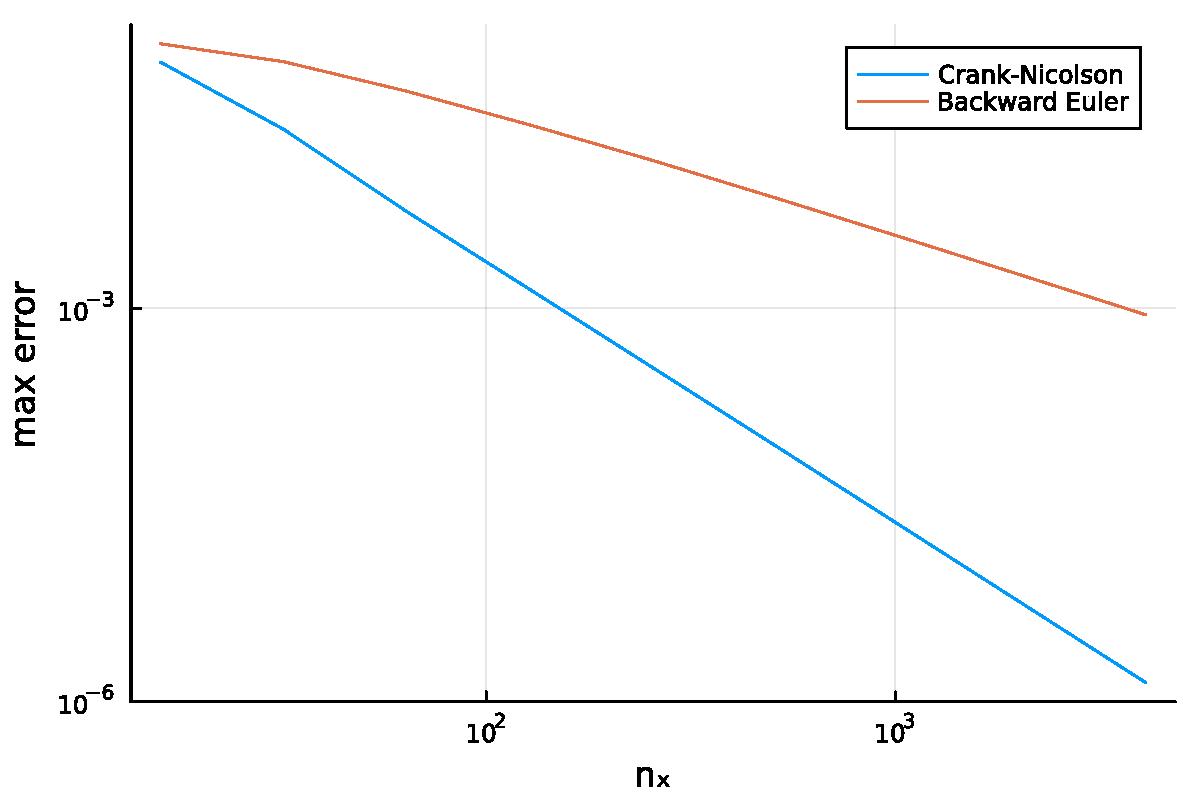
\includegraphics[width=\linewidth]{jl_6qsifB/Chapter5_Exercises_Solutions_6_1.pdf}

For the Crank-Nicolson method, we estimate the slope of the curve as follows:


\begin{lstlisting}
(*@\HLJLnf{log}@*)(*@\HLJLp{(}@*)(*@\HLJLn{cerr}@*)(*@\HLJLp{[}@*)(*@\HLJLk{end}@*)(*@\HLJLp{]}@*)(*@\HLJLoB{/}@*)(*@\HLJLn{cerr}@*)(*@\HLJLp{[}@*)(*@\HLJLk{end}@*)(*@\HLJLoB{-}@*)(*@\HLJLni{4}@*)(*@\HLJLp{])}@*)(*@\HLJLoB{/}@*)(*@\HLJLnf{log}@*)(*@\HLJLp{(}@*)(*@\HLJLn{nv}@*)(*@\HLJLp{[}@*)(*@\HLJLk{end}@*)(*@\HLJLp{]}@*)(*@\HLJLoB{/}@*)(*@\HLJLn{nv}@*)(*@\HLJLp{[}@*)(*@\HLJLk{end}@*)(*@\HLJLoB{-}@*)(*@\HLJLni{4}@*)(*@\HLJLp{])}@*)
\end{lstlisting}

\begin{lstlisting}
-1.9946564796544979
\end{lstlisting}


For the backward Euler method, the slope is approximately


\begin{lstlisting}
(*@\HLJLnf{log}@*)(*@\HLJLp{(}@*)(*@\HLJLn{berr}@*)(*@\HLJLp{[}@*)(*@\HLJLk{end}@*)(*@\HLJLp{]}@*)(*@\HLJLoB{/}@*)(*@\HLJLn{berr}@*)(*@\HLJLp{[}@*)(*@\HLJLk{end}@*)(*@\HLJLoB{-}@*)(*@\HLJLni{3}@*)(*@\HLJLp{])}@*)(*@\HLJLoB{/}@*)(*@\HLJLnf{log}@*)(*@\HLJLp{(}@*)(*@\HLJLn{nv}@*)(*@\HLJLp{[}@*)(*@\HLJLk{end}@*)(*@\HLJLp{]}@*)(*@\HLJLoB{/}@*)(*@\HLJLn{nv}@*)(*@\HLJLp{[}@*)(*@\HLJLk{end}@*)(*@\HLJLoB{-}@*)(*@\HLJLni{3}@*)(*@\HLJLp{])}@*)
\end{lstlisting}

\begin{lstlisting}
-0.9854061549915227
\end{lstlisting}


Hence, for the Crank-Nicolson method, the error decays as $\mathcal{O}(n_x^{-2})$ and for the backward Euler method, the error decays as $\mathcal{O}(n_x^{-1})$ as $n_x \to \infty$.



\end{document}
